\documentclass[journal]{IEEEtran}
\usepackage{graphicx}
\usepackage{amsmath}
\usepackage{booktabs}
\usepackage{url}
\usepackage{cite}
\usepackage{array}
\usepackage{multirow}

\title{Transformer-Based Low-Dose CT Image Denoising: A Comparative Study on AAPM-Mayo Data}

\author{Student Report for ECE448}

\begin{document}

\maketitle

\begin{abstract}
Low-dose computed tomography (LDCT) is clinically attractive because it can reduce radiation exposure, but lowering the X-ray dose also increases quantum noise and streak-like artifacts that may obscure anatomical structures. This report studies LDCT denoising as an artificial intelligence image restoration problem. The central question is whether recent Transformer-based restoration models provide a practical advantage over convolutional encoder-decoder baselines when applied to paired quarter-dose and full-dose CT slices. The report reviews several representative methods, including U-Net, RED-CNN, SwinIR, Restormer, and CTformer, and then evaluates reproduced experiments on the AAPM-Mayo low-dose CT data prepared as paired two-dimensional slices. The quantitative comparison uses peak signal-to-noise ratio (PSNR), structural similarity index (SSIM), and root mean square error (RMSE). In the local experiments, the original low-dose input achieves 29.2489 dB PSNR, 0.8759 SSIM, and 14.2416 RMSE on the held-out patient. Denoising models substantially improve image quality: CTRestormer at 11,500 iterations reaches 32.1294 dB PSNR and 0.8997 SSIM, CTformer reaches 32.3852 dB PSNR and 0.9026 SSIM, and RED-CNN reaches 32.6656 dB PSNR and 0.9067 SSIM. These results show that Transformer-based methods are effective for LDCT denoising, but also show that a well-trained convolutional residual baseline can remain highly competitive under limited training conditions. The discussion emphasizes that medical image denoising should be evaluated not only by numerical fidelity, but also by anatomical structure preservation, training cost, and the risk of smoothing diagnostically relevant details.
\end{abstract}

\begin{IEEEkeywords}
Low-dose CT, image denoising, medical image restoration, Transformer, RED-CNN, CTformer, Restormer.
\end{IEEEkeywords}

\section{Introduction}
Computed tomography (CT) is one of the most important imaging modalities in modern medicine because it provides detailed cross-sectional information about internal anatomical structures. However, CT imaging uses ionizing radiation, so repeated scans or scans for vulnerable patient groups raise safety concerns. A direct way to reduce patient risk is to lower the radiation dose, for example by reducing the tube current. The difficulty is that dose reduction degrades the acquired projection data and the reconstructed CT images. Low-dose CT images usually contain stronger noise, lower contrast visibility, and artifacts that can interfere with visual interpretation.

This trade-off creates a natural image restoration problem. Given a low-dose CT image, an algorithm should estimate an image that is close to the normal-dose or full-dose image while preserving anatomical boundaries and small structures. Traditional denoising methods often rely on handcrafted priors, local smoothing, non-local similarity, or iterative reconstruction. These approaches can be useful, but they may require careful parameter tuning and may struggle to model complex, spatially varying noise patterns. Deep learning changes the problem formulation by learning the mapping from low-dose images to full-dose images directly from paired data.

The present report focuses on supervised deep learning for LDCT denoising. The topic is clearly within artificial intelligence because it involves representation learning, optimization from paired data, and neural network architectures designed for inverse imaging problems. It is also clinically meaningful because improved denoising can support lower-dose imaging protocols, provided that the algorithm does not hallucinate structures or erase subtle lesions. The technical issue considered here is the architecture choice: convolutional residual encoder-decoder networks versus Transformer-based restoration networks.

Convolutional neural networks (CNNs) have long been successful in medical image restoration. U-Net introduced an encoder-decoder structure with skip connections for biomedical image segmentation, and the same multi-scale design principle has influenced many image restoration networks \cite{ronneberger2015unet}. RED-CNN, designed specifically for LDCT, uses convolutional and deconvolutional layers with residual skip connections and became a common LDCT denoising baseline \cite{chen2017redcnn}. More recently, Transformer architectures have become influential in image restoration. SwinIR applies shifted window self-attention to image restoration tasks \cite{liang2021swinir}. Restormer adapts Transformer blocks to high-resolution restoration through efficient attention and gated feed-forward layers \cite{zamir2022restormer}. CTformer further specializes Transformer ideas for LDCT denoising using a convolution-free Token2Token dilated vision Transformer design \cite{wang2023ctformer}.

The report is organized as follows. Section II reviews related work and explains why recent restoration Transformers are relevant to LDCT denoising. Section III describes the major algorithmic components. Section IV introduces the dataset, preprocessing, metrics, and experimental setup. Section V presents local quantitative and qualitative results. Section VI discusses the strengths, limitations, and practical implications of the observed results. Section VII concludes the report.

\section{Related Work}
\subsection{Low-Dose CT Datasets and Evaluation}
The AAPM-Mayo Low Dose CT Grand Challenge is a widely used benchmark for LDCT denoising research \cite{aapm2016ldct}. It provides paired normal-dose and simulated quarter-dose CT data. The availability of paired images makes supervised learning possible: a network can take the quarter-dose slice as input and use the full-dose slice as the regression target. Although full-dose CT is not a perfect noise-free ground truth, it is a clinically reasonable reference for learning and evaluation. The local experiments in this report use prepared AAPM-Mayo style data stored as normalized NumPy arrays.

LDCT denoising is commonly evaluated by PSNR, SSIM, RMSE, and visual comparison. PSNR measures pixel-level fidelity relative to the target; higher PSNR usually means lower average distortion. SSIM measures structural similarity and is often more aligned with perceived image quality. RMSE measures the magnitude of prediction error and is easier to interpret as a direct error measure. These metrics are useful but incomplete. A model can obtain high PSNR by oversmoothing, while a clinically useful image must preserve edges, textures, vessels, lesions, and organ boundaries.

\subsection{CNN-Based Denoising}
U-Net is a foundational encoder-decoder network in biomedical imaging \cite{ronneberger2015unet}. Its key idea is to combine a contracting path, which captures semantic and contextual information, with an expanding path, which recovers spatial resolution. Skip connections transfer high-resolution features from the encoder to the decoder. Although U-Net was proposed for segmentation, its structure is natural for denoising because the output must align pixel-by-pixel with the input.

RED-CNN is more directly related to LDCT denoising \cite{chen2017redcnn}. It uses a residual encoder-decoder CNN to learn the difference between noisy low-dose images and normal-dose references. The residual formulation is important because the low-dose image already contains most anatomical content; the network should mainly remove noise and artifacts rather than synthesize a completely new image. Residual learning also improves optimization because the model learns a correction term instead of a full image from scratch. RED-CNN remains a strong baseline because convolution is well matched to local image statistics and because the architecture is relatively compact.

\subsection{Transformer-Based Image Restoration}
Transformers were originally developed for sequence modeling, but self-attention is attractive for image restoration because it can model long-range dependencies. A noisy CT pixel should be interpreted not only from its immediate neighborhood, but also from repeated anatomical patterns, symmetric structures, and broader contextual cues. However, standard global self-attention is expensive for high-resolution images because its memory and computation scale quadratically with the number of tokens.

SwinIR addresses this problem by using the Swin Transformer structure, which computes self-attention inside local windows and shifts the windows across layers \cite{liang2021swinir}. This makes Transformer restoration practical for images while still allowing cross-window information flow. Restormer proposes another efficient design for high-resolution restoration. It uses multi-Dconv head transposed attention (MDTA) and a gated-Dconv feed-forward network (GDFN), combining attention with depthwise convolutional operations that preserve local inductive bias \cite{zamir2022restormer}. These design choices are relevant to LDCT because medical images are high-resolution and require both local texture handling and broader structural modeling.

CTformer specializes the Transformer idea for LDCT denoising \cite{wang2023ctformer}. It uses Token2Token processing and dilated attention mechanisms to enhance local-global feature extraction without relying on a conventional CNN backbone. This makes CTformer a representative medical imaging Transformer rather than only a general natural image restoration method. In this report, CTformer is treated as the main reproduced Transformer baseline, while a Restormer-inspired CTRestormer variant is treated as an additional experimental model.

\section{Technical Algorithms}
\subsection{Problem Formulation}
Let $x$ denote a low-dose CT slice and $y$ denote the corresponding full-dose CT slice. A supervised denoising model learns a mapping
\begin{equation}
\hat{y}=f_{\theta}(x),
\end{equation}
where $\theta$ represents trainable parameters. The training objective minimizes the discrepancy between $\hat{y}$ and $y$. A simple objective is mean squared error,
\begin{equation}
\mathcal{L}_{MSE}=\frac{1}{N}\sum_{i=1}^{N}(\hat{y}_{i}-y_{i})^2,
\end{equation}
but many image restoration systems also use structural or perceptual terms. In the local CTRestormer experiment, a hybrid loss combining Charbonnier loss and an SSIM-related term was used. The motivation is to improve both pixel fidelity and structure preservation.

The desired mapping is close to identity because the low-dose input already contains the correct anatomy. Therefore, many denoising models use residual learning:
\begin{equation}
\hat{y}=x+r_{\theta}(x),
\end{equation}
where $r_{\theta}(x)$ predicts the residual correction. This formulation encourages the network to focus on noise and artifact removal rather than rebuilding the entire image.

\subsection{Residual Encoder-Decoder CNN}
RED-CNN represents the CNN approach. Convolutional layers encode local image features, while deconvolutional or upsampling layers recover the image resolution. Skip connections preserve low-level details and support gradient flow. The main strength of this family is its local inductive bias. CT noise and edges are often local, so convolutional filters can efficiently learn denoising patterns. CNNs are also computationally efficient and easier to train with limited data.

The weakness is that standard convolutions have limited receptive fields unless the network is deep or uses dilation and multi-scale mechanisms. Some artifacts and anatomical structures span large regions. A CNN can model them, but it may need many layers or carefully designed skip connections. This limitation motivates attention-based models.

\subsection{Window and Hierarchical Transformers}
Transformer restoration models convert images or feature maps into token representations and use attention to aggregate information. For image restoration, a model must maintain spatial precision. SwinIR solves the cost problem by computing attention inside windows. Shifted windows then allow neighboring windows to exchange information across layers. This design gives the model more contextual reasoning than a purely local convolution while controlling computation.

Restormer uses a different strategy. Instead of applying expensive global spatial attention directly, it computes attention in a transposed channel-oriented manner and uses depthwise convolution to preserve local spatial interactions. Its GDFN block uses gating to control information flow through the feed-forward network. This is especially appropriate for restoration because the model should selectively suppress noise while retaining meaningful structures.

\subsection{CTformer and CTRestormer}
CTformer applies a convolution-free Transformer design to LDCT denoising. Token2Token modules progressively structure the token representation, and dilated attention enlarges the effective context. The central idea is that CT denoising benefits from both local detail and non-local anatomical context. A pelvis CT slice, for example, contains repeated texture in soft tissue, sharp bone boundaries, and large homogeneous regions. A Transformer can in principle compare distant features and use context to distinguish noise from structure.

The local CTRestormer model follows the Restormer restoration philosophy. It uses overlap patch embedding, a multi-scale encoder-decoder hierarchy, Transformer blocks with layer normalization, MDTA-style attention, GDFN-style feed-forward modules, and residual output. The model was configured for a 6GB NVIDIA RTX 3060 Laptop GPU, so its width and block counts were reduced compared with larger restoration models. This resource constraint is important: a Transformer can be powerful but may need longer training or larger capacity to outperform a compact CNN baseline.

\begin{figure*}[t]
\centering
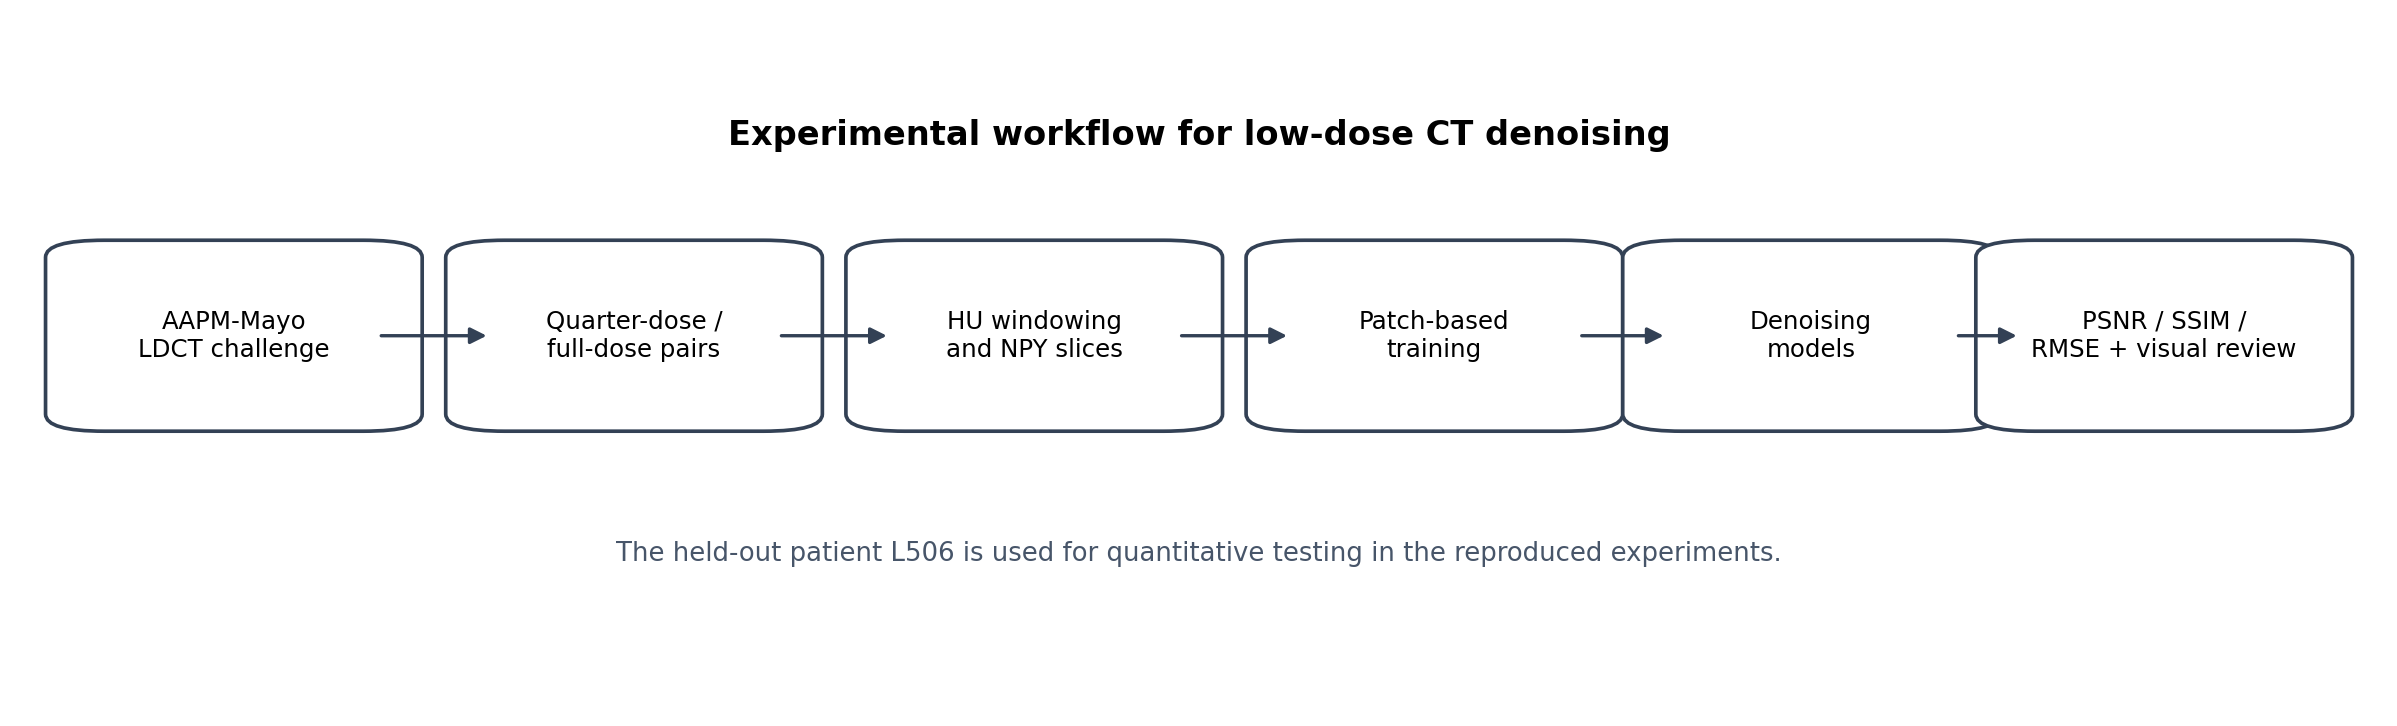
\includegraphics[width=0.95\textwidth]{figures/experimental_workflow.png}
\caption{Experimental workflow used in this report. Paired quarter-dose and full-dose CT slices are prepared as normalized NPY arrays, trained with patch-based sampling, and evaluated using PSNR, SSIM, RMSE, and visual comparison.}
\label{fig:workflow}
\end{figure*}

\begin{figure*}[t]
\centering
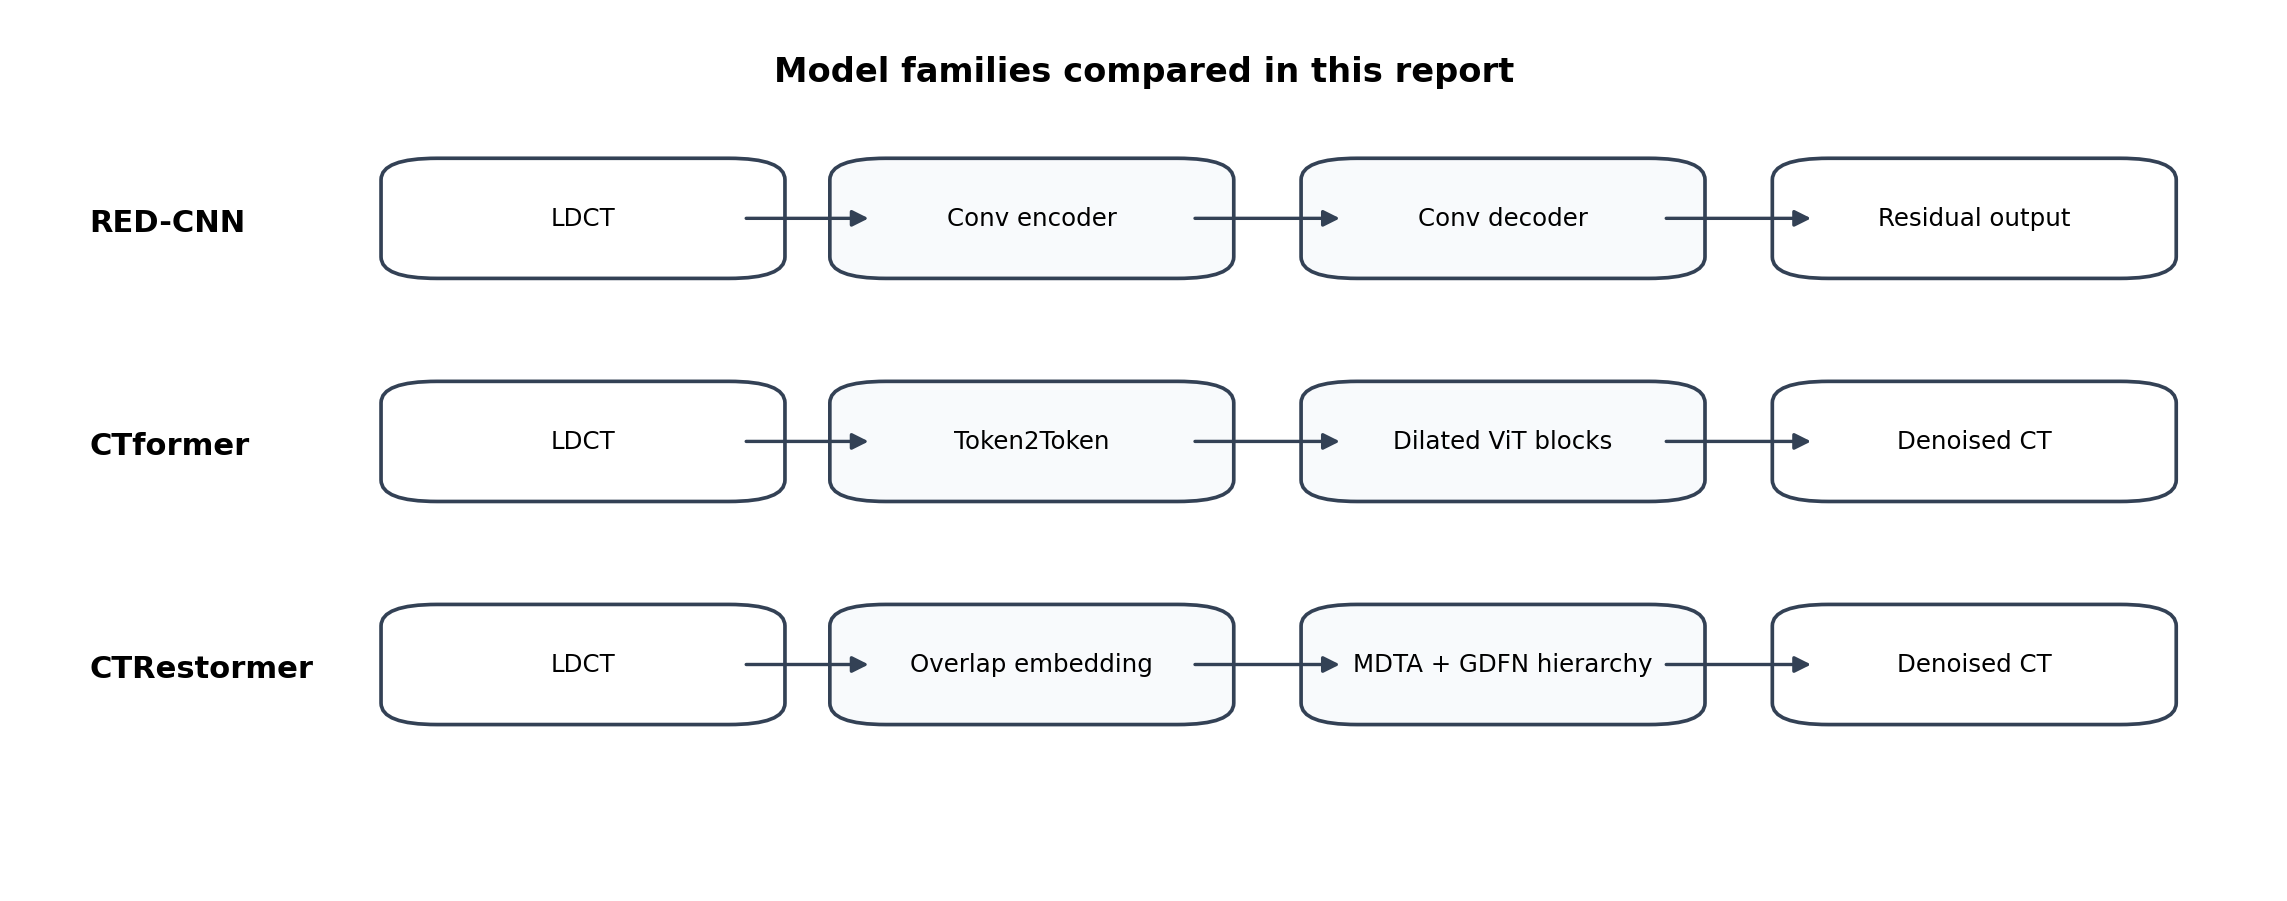
\includegraphics[width=0.90\textwidth]{figures/model_comparison_schematic.png}
\caption{High-level comparison of the model families discussed in the report. RED-CNN is a convolutional residual encoder-decoder, CTformer uses Token2Token and dilated Transformer blocks, and CTRestormer follows a Restormer-style hierarchical image restoration design.}
\label{fig:model_schematic}
\end{figure*}

\section{Experimental Setup}
\subsection{Dataset}
The experiments use a prepared AAPM-Mayo style LDCT dataset stored in \texttt{npy\_img\_3mm\_B30}. The local dataset contains 2,378 paired input slices from ten patient IDs: L067, L096, L109, L143, L192, L286, L291, L310, L333, and L506. Each sample consists of a quarter-dose input image and a full-dose target image. The arrays are normalized two-dimensional CT slices of size $512\times512$.

The held-out testing patient in the reproduced experiments is L506. This patient-level split is important because testing on slices from a patient seen during training could overestimate performance. By evaluating on a held-out patient, the test more closely measures whether the learned denoising behavior transfers to unseen anatomy from a different scan.

\subsection{Training and Models}
The reproduced CTformer experiment uses patch-based training with the prepared LDCT slices. The model was trained for 100 epochs in the available local run, saving checkpoints and loss curves. The CTformer result reported here corresponds to the reproduced run in \texttt{runs/train\_100ep\_bs4}.

The RED-CNN baseline was evaluated separately and is included because it is a classic LDCT denoising baseline. The CTRestormer model was trained as a Restormer-inspired Transformer variant. Its 11,500-iteration checkpoint was evaluated, but the training was only about 5.3\% of the planned long schedule. Therefore, its result should be interpreted as an early-stage result rather than a fully converged result. The CTRestormer configuration used a reduced dimension, mixed precision, AdamW optimization, cosine learning rate scheduling, gradient accumulation, and a hybrid restoration loss.

\subsection{Metrics}
Three metrics are reported. PSNR is computed from the mean squared error and is measured in decibels. SSIM measures luminance, contrast, and structural similarity between the denoised image and the full-dose target. RMSE measures average pixel error magnitude. Higher PSNR and SSIM are better, while lower RMSE is better. The metrics are averaged over the held-out test slices.

\section{Results}
\subsection{Quantitative Comparison}
Table \ref{tab:metrics} shows the main quantitative comparison. All denoising models substantially improve over the original low-dose input. The low-dose input has 29.2489 dB PSNR and 0.8759 SSIM. CTRestormer improves this to 32.1294 dB PSNR and 0.8997 SSIM at 11,500 iterations. CTformer improves further to 32.3852 dB PSNR and 0.9026 SSIM. RED-CNN achieves the best local result among the compared methods, with 32.6656 dB PSNR, 0.9067 SSIM, and 9.4867 RMSE.

\begin{table}[t]
\centering
\caption{Quantitative LDCT denoising results on the held-out L506 test patient.}
\label{tab:metrics}
\begin{tabular}{lccc}
\toprule
Method & PSNR $\uparrow$ & SSIM $\uparrow$ & RMSE $\downarrow$ \\
\midrule
Low-dose input & 29.2489 & 0.8759 & 14.2416 \\
CTRestormer, 11,500 iters & 32.1294 & 0.8997 & 10.0689 \\
CTformer & 32.3852 & 0.9026 & 9.8366 \\
RED-CNN & 32.6656 & 0.9067 & 9.4867 \\
\bottomrule
\end{tabular}
\end{table}

\begin{figure*}[t]
\centering
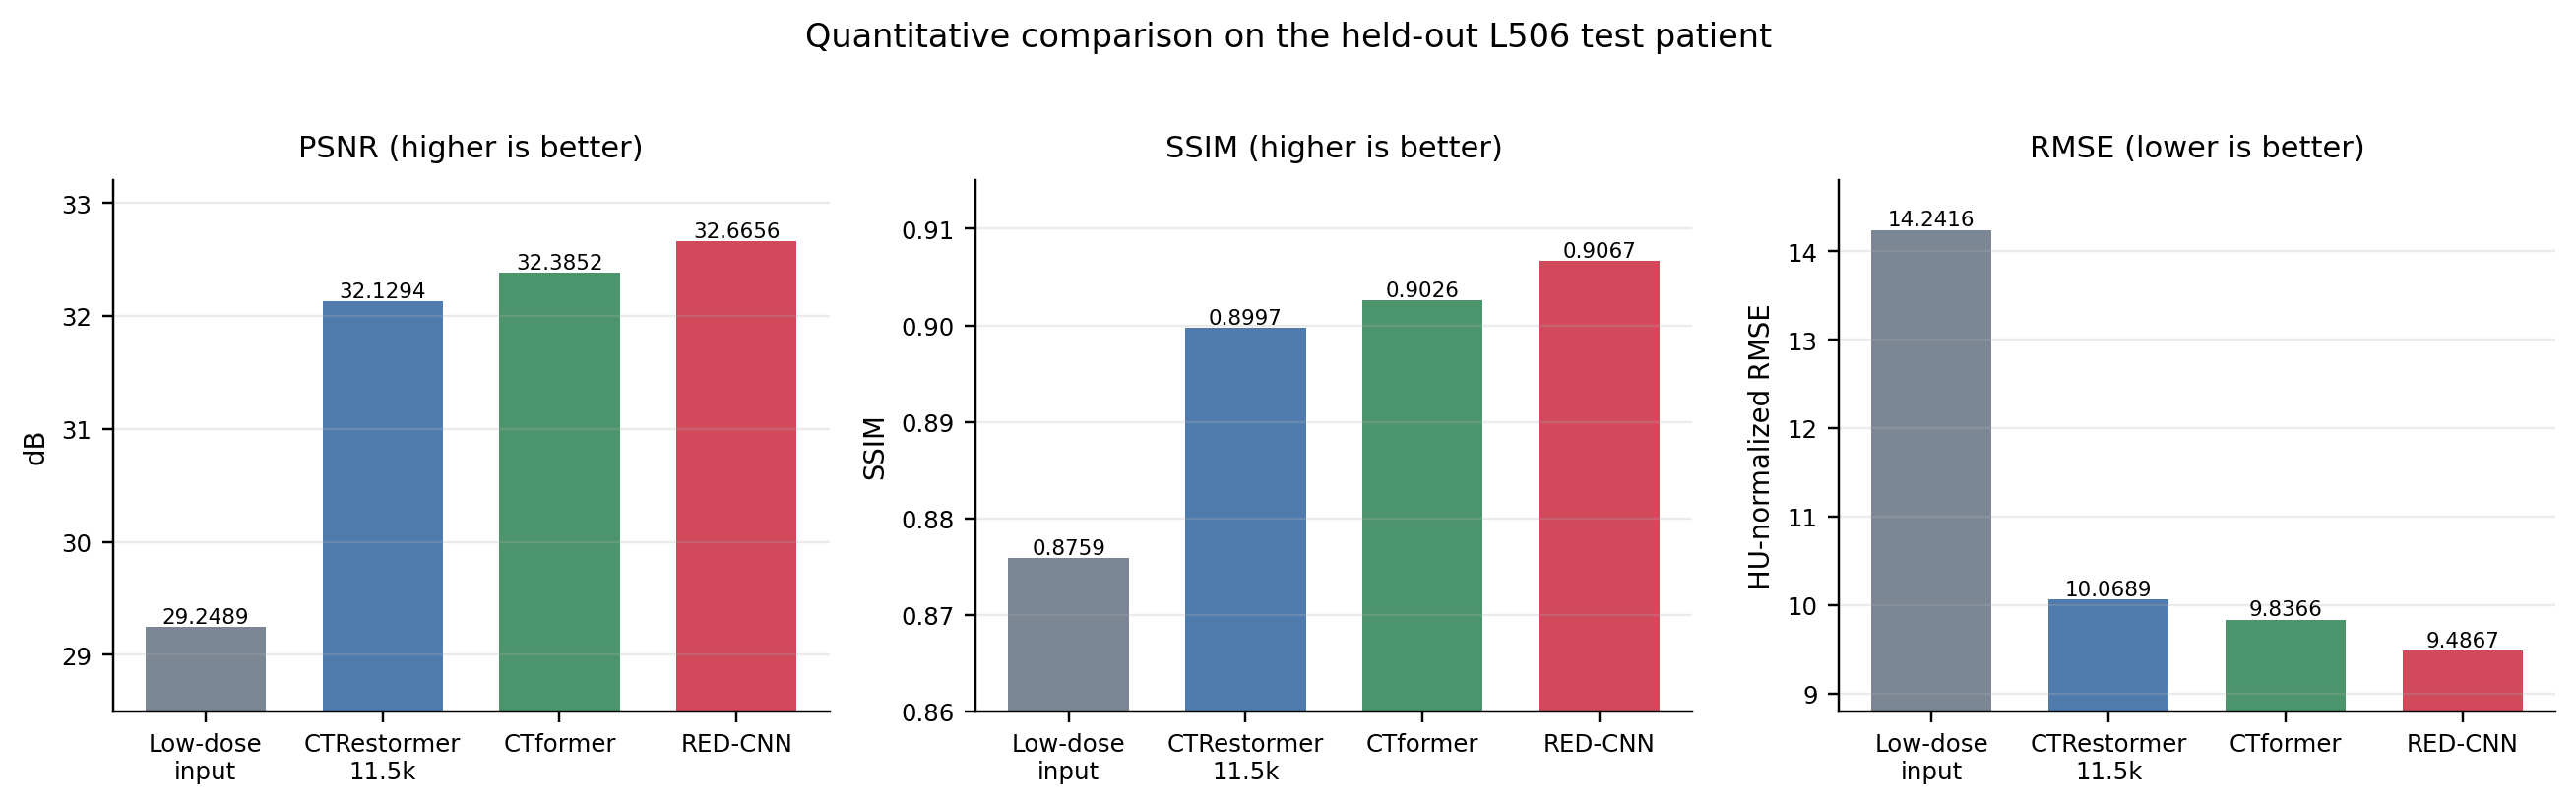
\includegraphics[width=0.95\textwidth]{figures/metrics_comparison.png}
\caption{Metric comparison on the held-out L506 patient. The low-dose input is clearly improved by all denoising models. In the reproduced local results, RED-CNN remains the strongest baseline, while CTformer is close and CTRestormer is effective but still early in training.}
\label{fig:metrics}
\end{figure*}

The PSNR gain from low-dose input to CTformer is approximately 3.14 dB, and the RMSE decreases from 14.2416 to 9.8366. This is a meaningful improvement because CT images are sensitive to subtle intensity changes. CTRestormer also improves the input by about 2.88 dB PSNR. Its slightly weaker performance compared with CTformer and RED-CNN is not surprising because its reported checkpoint is early. Transformer restoration models often require long training to stabilize, especially when adapted to a medical dataset with limited patient diversity.

\subsection{Training Trend}
Figure \ref{fig:loss} shows the CTformer training loss trend from the reproduced training run. The curve decreases over time and reaches a low-loss region near the end of training. This trend supports the validity of the reproduced model: the network learned a stable mapping from quarter-dose to full-dose slices rather than producing random outputs. However, the loss curve alone cannot prove clinical quality. It should be interpreted together with test metrics and visual examples.

\begin{figure}[t]
\centering
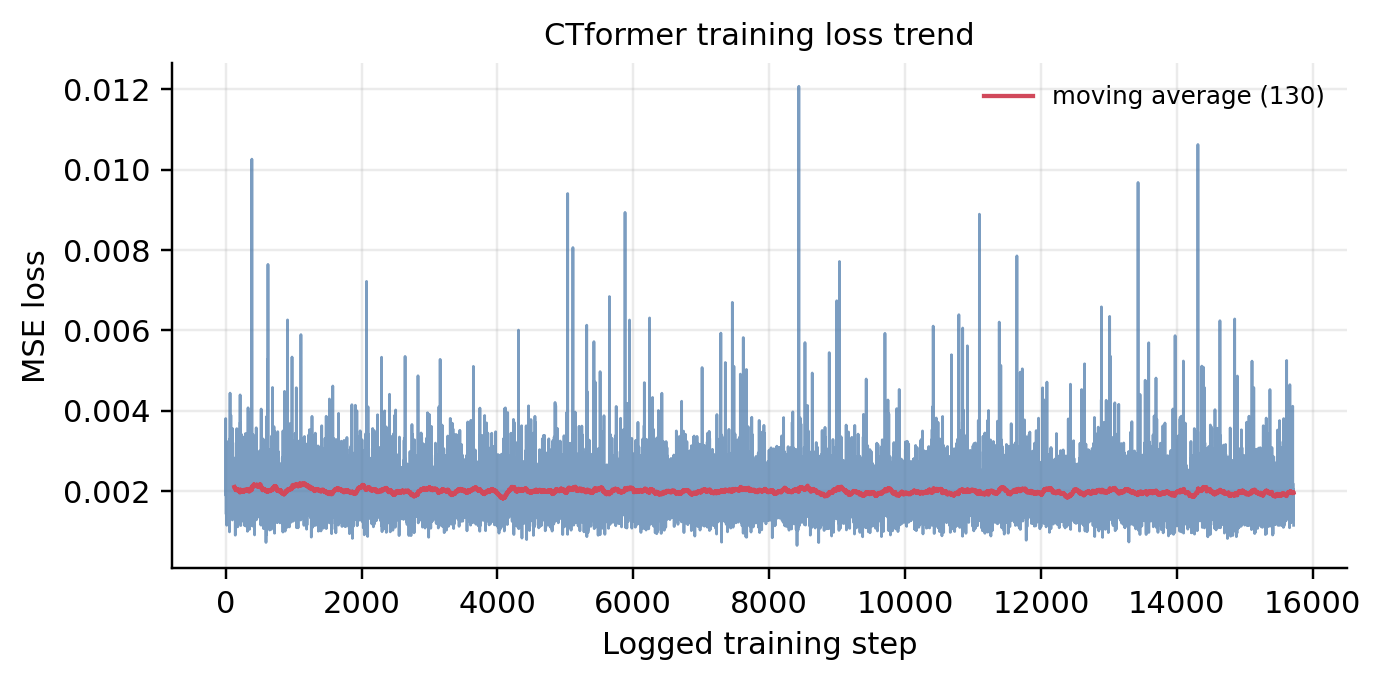
\includegraphics[width=0.48\textwidth]{figures/ctformer_loss_curve.png}
\caption{Training loss trend from the reproduced CTformer run. The smoothed curve shows convergence toward a low-loss region.}
\label{fig:loss}
\end{figure}

\subsection{Qualitative Observation}
Figure \ref{fig:qualitative} shows a representative L506 slice. The quarter-dose input contains visibly stronger grain-like noise in soft tissue regions. The model output is smoother and closer to the full-dose target. The single-slice metrics shown in the figure also improve from the quarter-dose input to the denoised result. The qualitative result illustrates the main benefit of deep learning denoising: noise suppression without simply blurring the entire image.

\begin{figure*}[t]
\centering
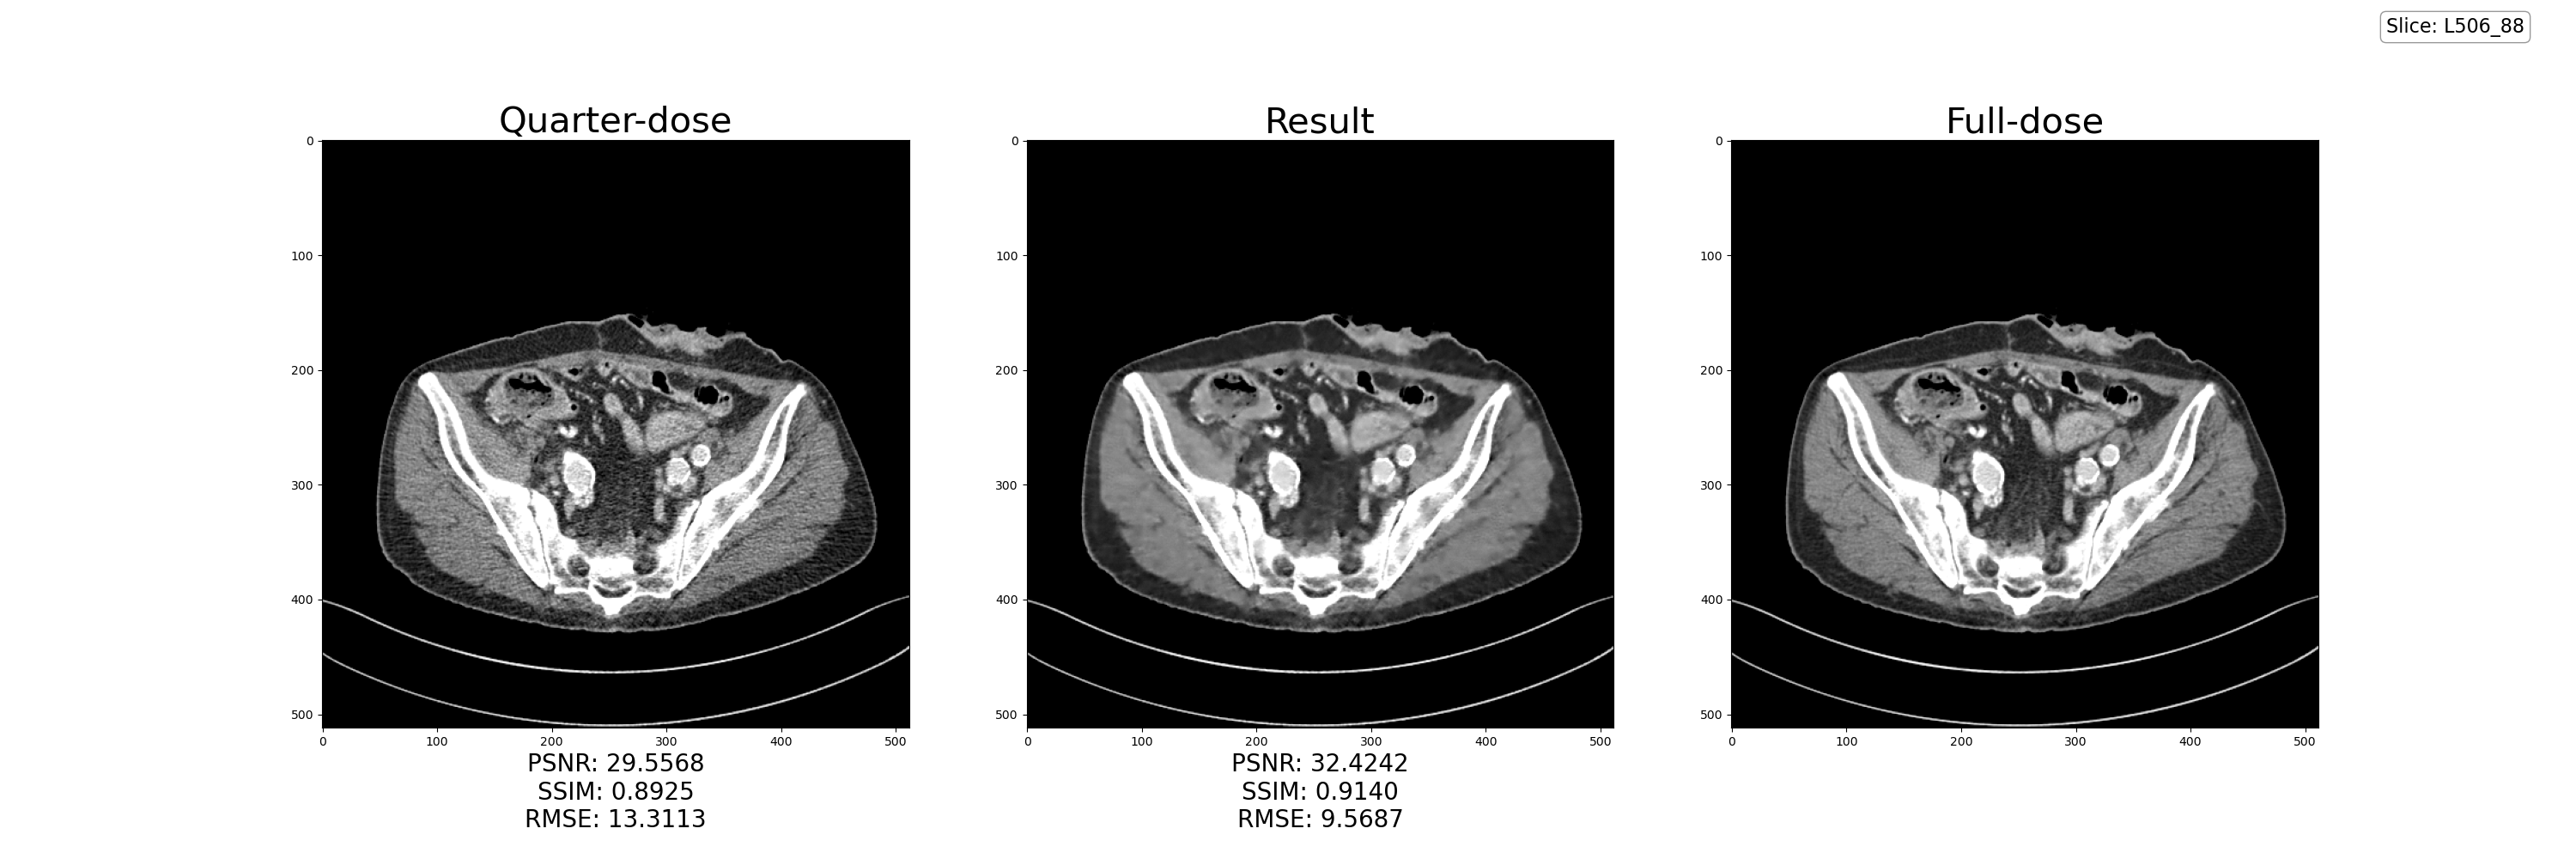
\includegraphics[width=0.98\textwidth]{figures/qualitative_l506_88_ctformer.png}
\caption{Representative qualitative CTformer result for slice L506\_88. The denoised result reduces visible noise compared with the quarter-dose input and approaches the full-dose reference.}
\label{fig:qualitative}
\end{figure*}

At the same time, the output appears slightly smoother than the full-dose target in some regions. This is a common issue in supervised denoising. If the loss emphasizes average pixel accuracy, the model may remove high-frequency content that resembles noise. In medical imaging, this is not merely an aesthetic issue. Fine structures can be diagnostically important, and oversmoothing can reduce confidence in subtle findings. Therefore, denoising models should be judged by both numerical metrics and careful visual review.

\section{Discussion}
The first important observation is that the LDCT denoising problem is learnable from paired data. Every learned model improves PSNR, SSIM, and RMSE compared with the low-dose input. This confirms that the low-dose image contains enough information for a neural network to estimate a cleaner image, and that paired full-dose supervision provides a useful training signal.

The second observation is that Transformer models are effective but not automatically superior. CTformer performs close to RED-CNN but does not exceed it in the local reproduced results. CTRestormer also improves the input substantially, but its early checkpoint lags behind the stronger baselines. This does not mean Transformer models are unsuitable for LDCT. Instead, it shows that architecture alone is not enough. Training schedule, model scale, loss design, data split, preprocessing, and GPU constraints all matter. A compact CNN that is well matched to local denoising statistics can outperform a larger attention model if the Transformer is undertrained or reduced too aggressively.

The result is also consistent with the nature of CT denoising. Much of the noise is local and texture-like, so convolutional filters are very effective. Attention becomes more valuable when non-local context is needed, for example to maintain consistency across repeated anatomical structures or distinguish low-contrast structure from random noise. The best practical systems may combine convolutional inductive bias with attention rather than treating CNNs and Transformers as mutually exclusive categories. Restormer itself reflects this idea by using depthwise convolution inside Transformer blocks.

Another issue is data scale. The local dataset contains many slices but only ten patients. Adjacent slices from the same patient are highly correlated, so the effective diversity is smaller than the raw slice count suggests. Transformers often benefit from larger and more diverse datasets because attention-based models have weaker built-in local assumptions than CNNs. For a small medical dataset, strong regularization, patch augmentation, careful normalization, and patient-level validation are essential.

The evaluation also has limitations. PSNR and SSIM compare images against full-dose references, but full-dose CT still contains noise and may not be a perfect anatomical ground truth. Metrics can reward smoothing because smoothing reduces pixel variance. Clinical utility requires more than similarity to a reference image. A future study should include radiologist assessment, lesion detectability analysis, noise power spectrum, edge preservation measures, or task-specific downstream evaluation. For example, if a denoised image improves PSNR but reduces visibility of a small lesion, the algorithm would be unsafe despite a good numerical score.

For the current course report, however, the experiment is sufficient to demonstrate algorithm testing with actual data. It uses real paired LDCT data, reproduces multiple model results, reports standard metrics, and includes visual analysis. The results support a balanced conclusion: Transformer-based LDCT denoising is a promising research direction, but CNN residual baselines remain important and should not be dismissed. The most reliable research claim is not that one architecture universally wins, but that each architecture encodes a different trade-off between local bias, global context, training cost, and detail preservation.

\section{Conclusion}
This report studied low-dose CT denoising as an AI-based medical image restoration problem. It reviewed CNN and Transformer approaches, including U-Net, RED-CNN, SwinIR, Restormer, and CTformer, and evaluated reproduced experiments on prepared AAPM-Mayo LDCT data. The local results show that learned denoising models significantly improve over the quarter-dose input. RED-CNN achieved the best reported local metrics, CTformer was close, and CTRestormer showed promising early-stage denoising but had not yet surpassed the baselines at 11,500 iterations.

The main conclusion is that Transformer-based restoration models are valuable for LDCT because they can model broader context than purely local convolution. However, their practical advantage depends on sufficient training, appropriate model size, and careful evaluation. In medical imaging, denoising should preserve anatomical truth rather than merely produce visually smooth images. Future work should continue CTRestormer training, compare checkpoints under the same test protocol, add more patient-level validation, and include clinical or task-oriented measures of image quality.

\begin{thebibliography}{99}

\bibitem{aapm2016ldct}
American Association of Physicists in Medicine, ``Low Dose CT Grand Challenge,'' 2016. [Online]. Available: \url{https://www.aapm.org/GrandChallenge/LowDoseCT/}

\bibitem{ronneberger2015unet}
O. Ronneberger, P. Fischer, and T. Brox, ``U-Net: Convolutional networks for biomedical image segmentation,'' in \emph{Proc. Medical Image Computing and Computer-Assisted Intervention (MICCAI)}, 2015, pp. 234--241.

\bibitem{chen2017redcnn}
H. Chen, Y. Zhang, M. K. Kalra, F. Lin, Y. Chen, P. Liao, J. Zhou, and G. Wang, ``Low-dose CT with a residual encoder-decoder convolutional neural network,'' \emph{IEEE Transactions on Medical Imaging}, vol. 36, no. 12, pp. 2524--2535, 2017.

\bibitem{liang2021swinir}
J. Liang, J. Cao, G. Sun, K. Zhang, L. Van Gool, and R. Timofte, ``SwinIR: Image restoration using Swin Transformer,'' in \emph{Proc. IEEE/CVF International Conference on Computer Vision Workshops}, 2021, pp. 1833--1844.

\bibitem{zamir2022restormer}
S. W. Zamir, A. Arora, S. Khan, M. Hayat, F. S. Khan, M. Yang, and L. Shao, ``Restormer: Efficient Transformer for high-resolution image restoration,'' in \emph{Proc. IEEE/CVF Conference on Computer Vision and Pattern Recognition}, 2022, pp. 5728--5739.

\bibitem{wang2022uformer}
Z. Wang, X. Cun, J. Bao, W. Zhou, J. Liu, and H. Li, ``Uformer: A general U-shaped Transformer for image restoration,'' in \emph{Proc. IEEE/CVF Conference on Computer Vision and Pattern Recognition}, 2022, pp. 17683--17693.

\bibitem{wang2023ctformer}
D. Wang, F. Fan, Z. Wu, R. Liu, F. Wang, and H. Yu, ``CTformer: Convolution-free Token2Token dilated vision Transformer for low-dose CT denoising,'' \emph{Physics in Medicine \& Biology}, vol. 68, no. 6, 2023.

\end{thebibliography}

\end{document}
